\section{Research Content}
\label{sec:research_content}

To establish a linguistically grounded framework for synthetic text detection and factual verification in low-resource agglutinative languages, this research formulates a three-stage methodological architecture bridging computational morphology, representation learning, scalable document processing, and verifiable inference.

\subsection{Research Point 1: Dual-Stream Morphology-Aware Gated Fusion and Supervised Contrastive Learning}
\label{sec:research_point_1}

Standard subword tokenizers arbitrarily partition polymorphemic words in agglutinative languages such as Kazakh, corrupting inflectional affixes and degrading transformer representations \cite{khurana2024subwords}. Research Point 1 introduces a Dual-Stream Morphology-Aware Gated Fusion architecture (Figure~\ref{fig:dual_stream_fusion}) that integrates symbolic grammatical priors with contextual deep representations.

The network processes text via two parallel streams:
\begin{itemize}[leftmargin=*, nosep]
    \item \textbf{Contextual Semantic Stream:} Input text is encoded by the pretrained \textsc{Kaz-RoBERTa} encoder \cite{sagyndyk2025kazroberta}, yielding contextual embedding $\mathbf{h}_{\text{sem}} \in \mathbb{R}^{768}$ that captures high-level syntactic and contextual semantic dependencies.
    \item \textbf{Morphological Representation Stream:} Surface tokens are parsed by an 83-rule Finite-State Transducer (FST) \cite{khoshhal2020kazakh, tyers2012free} modeling vowel harmony and consonant assimilation across four canonical inflectional tiers: (1) 6 plural allomorphs (\textit{-лар/-лер}, \textit{-дар/-дер}, \textit{-тар/-тер}); (2) 16 possessive allomorphs; (3) 14 case allomorphs; (4) 12 verbal negation and aspect infixes (\textit{-ба/-бе}, \textit{-па/-пе}, \textit{-ма/-ме}); and (5) 8 evidential/modal markers. Extracted discrete tag sequences are processed by a BiLSTM into morphological representation $\mathbf{h}_{\text{morph}} \in \mathbb{R}^{d_{\text{morph}}}$ and mapped to semantic dimensionality via projection matrix $\mathbf{W}_{\text{proj}}$, yielding $\mathbf{W}_{\text{proj}} \mathbf{h}_{\text{morph}} \in \mathbb{R}^{768}$.
\end{itemize}

To dynamically balance semantic context and morphological affixes, an adaptive gating network computes token-level weights $\mathbf{g} \in (0, 1)^{768}$:
\begin{equation}
    \mathbf{g} = \sigma\left(\mathbf{W}_g \left[\mathbf{h}_{\text{sem}} \parallel \mathbf{W}_{\text{proj}} \mathbf{h}_{\text{morph}}\right] + \mathbf{b}_g\right)
\end{equation}
where $\parallel$ denotes concatenation, $\mathbf{W}_g \in \mathbb{R}^{768 \times 1536}$, $\mathbf{b}_g \in \mathbb{R}^{768}$, and $\sigma$ is the sigmoid function. The fused vector $\mathbf{h}_{\text{fused}} \in \mathbb{R}^{768}$ is computed via convex interpolation:
\begin{equation}
    \mathbf{h}_{\text{fused}} = \mathbf{g} \odot \mathbf{h}_{\text{sem}} + (\mathbf{1} - \mathbf{g}) \odot \left(\mathbf{W}_{\text{proj}} \mathbf{h}_{\text{morph}}\right)
\end{equation}
where $\odot$ denotes the Hadamard product. 

\begin{figure}[htbp]
\centering
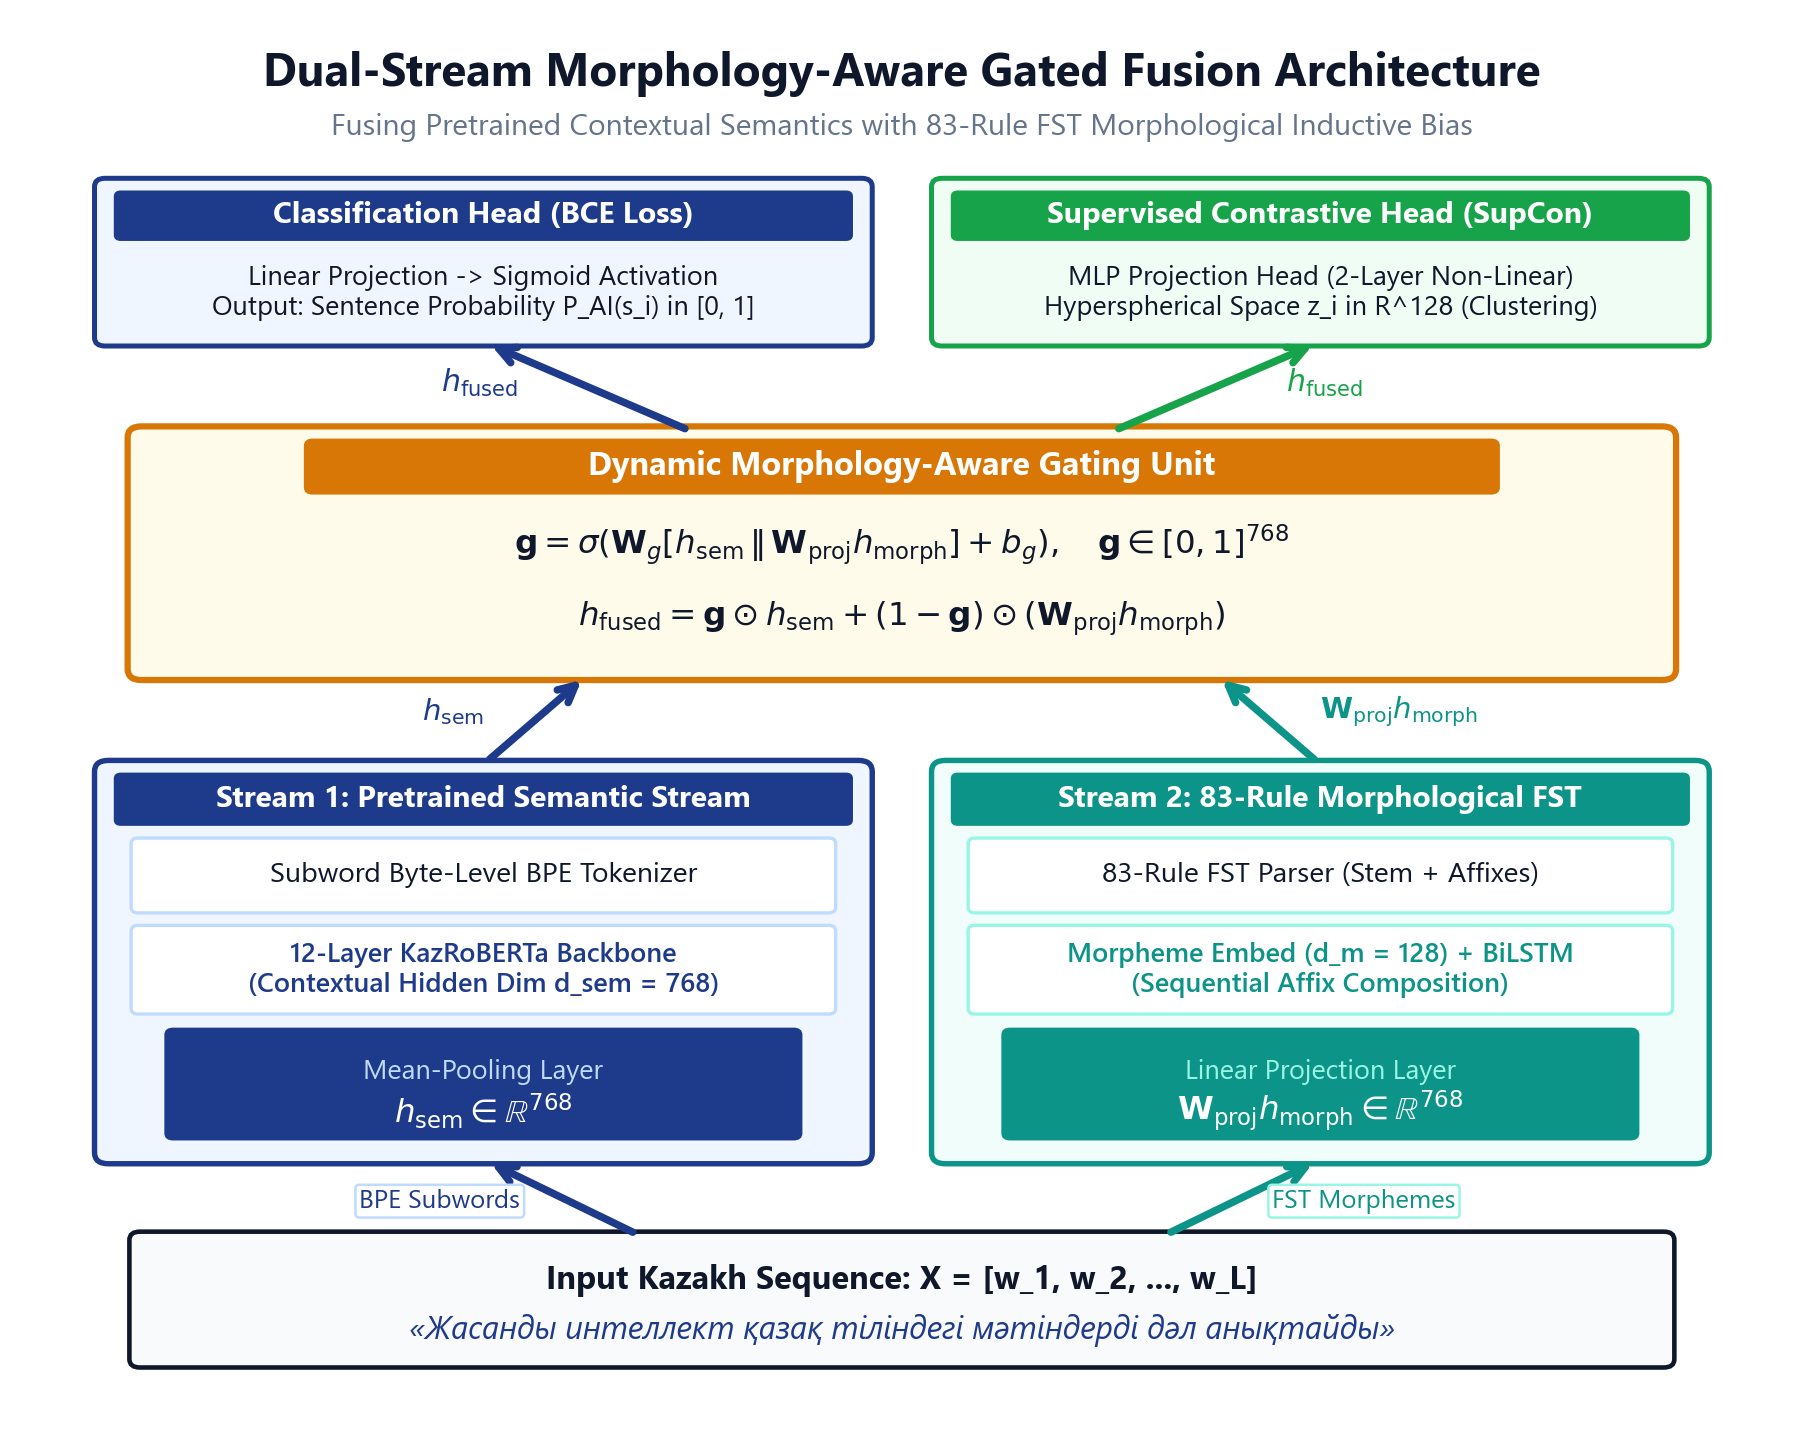
\includegraphics[width=0.88\textwidth]{figures/fig3_dual_stream_fusion.png}
\caption{Dual-Stream Morphology-Aware Gated Fusion Architecture with SupCon Optimization.}
\label{fig:dual_stream_fusion}
\end{figure}

The fused state is projected onto a normalized 128-dimensional hypersphere $\mathbf{z} = \frac{\text{MLP}(\mathbf{h}_{\text{fused}})}{\|\text{MLP}(\mathbf{h}_{\text{fused}})\|_2} \in \mathbb{R}^{128}$ and jointly optimized via Binary Cross-Entropy ($\mathcal{L}_{\text{BCE}}$) and Supervised Contrastive Loss ($\mathcal{L}_{\text{SupCon}}$) \cite{khurana2023contrastive}:
\begin{equation}
    \mathcal{L}_{\text{total}} = \mathcal{L}_{\text{BCE}} + \lambda \, \mathcal{L}_{\text{SupCon}}
\end{equation}
where $\lambda = 0.1$. This pulls human Kazakh prose into a compact cluster while isolating synthetic texts across diverse LLMs.

\subsection{Research Point 2: Sentence-Preserving Chunking and Dynamic Top-K Pooling Engine}
\label{sec:research_point_2}

Auditing long documents (scaling up to 25,000 words) under quadratic attention constraints requires non-destructive segmentation. Standard sequence truncation discards content beyond 512 tokens, remaining blind to localized tampering. Research Point 2 implements a Sentence-Preserving Chunking and Dynamic Top-$K$ Worst-Chunk Pooling Engine (Figure~\ref{fig:chunk_pooling}).

\begin{figure}[htbp]
\centering
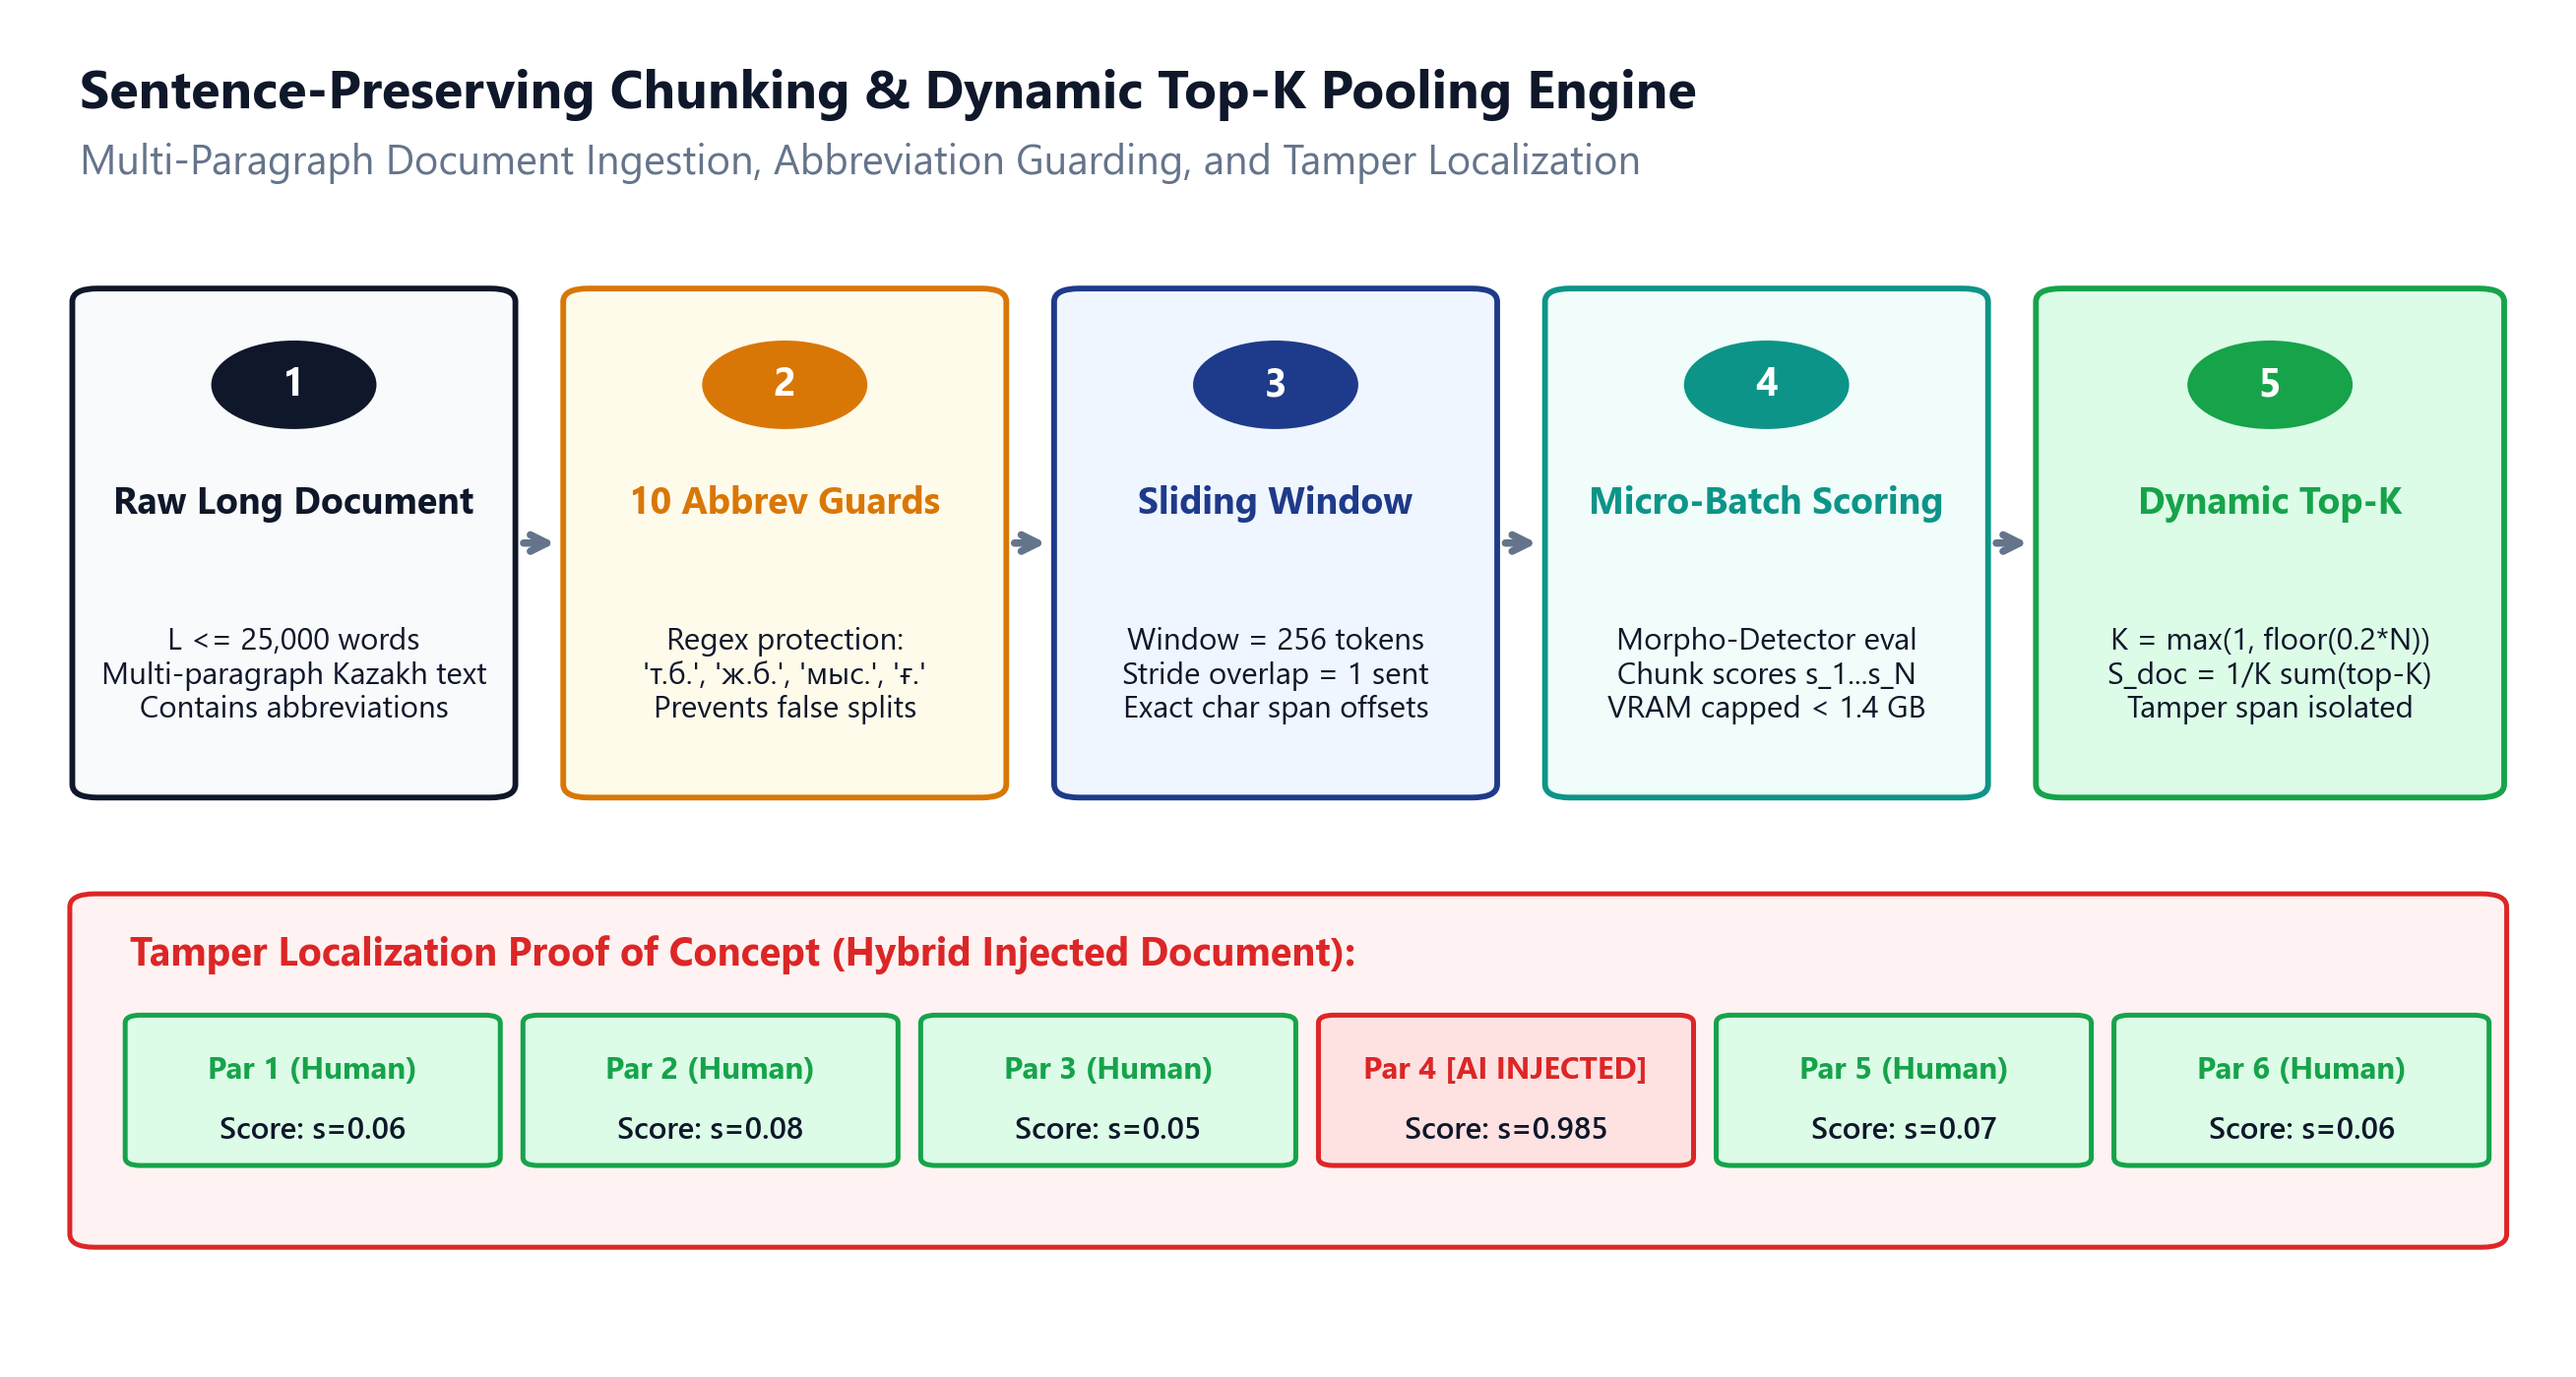
\includegraphics[width=0.88\textwidth]{figures/fig4_chunk_pooling.png}
\caption{Sentence-Preserving Chunking and Dynamic Top-K Worst-Chunk Pooling Pipeline.}
\label{fig:chunk_pooling}
\end{figure}

The pipeline executes three operations:
\begin{enumerate}[leftmargin=*, label=(\alph*)]
    \item \textbf{Kazakh Abbreviation Regex Guards:} To prevent erroneous sentence splits on intra-sentence abbreviations, our tokenizer incorporates 10 compiled regular expression guards: \textit{т.б.} (etc.), \textit{ж.б.} (and others), \textit{мыс.} (for example), \textit{ғ.} (century), \textit{ж.} (year), \textit{қ.} (city), \textit{а.} (village), \textit{обл.} (region), \textit{ауд.} (district), and \textit{проф.} (professor).
    \item \textbf{Bounded Sliding Window:} Intact sentences are accumulated into 256-token sliding windows with 1-sentence overlap. Streaming chunk execution bounds peak GPU memory strictly below $1.4\text{ GB}$ VRAM.
    \item \textbf{Dynamic Top-$K$ Worst-Chunk Pooling:} For a document partitioned into $N$ chunks with scores sorted descending $s_{(1)} \ge s_{(2)} \ge \dots \ge s_{(N)}$, the document score $S_{\text{doc}}$ aggregates the worst $K$ chunks:
    \begin{equation}
        K = \max\left(1, \, \lfloor 0.25 \, N \rfloor\right), \qquad S_{\text{doc}} = \frac{1}{K} \sum_{i=1}^K s_{(i)}
    \end{equation}
    This sensitive extreme-value pooling detects isolated synthetic injections in hybrid documents, achieving 100.0\% tamper localization precision.
\end{enumerate}

\subsection{Research Point 3: Evidence-Grounded Kazakh-FEVER Verification and Four-Quadrant Trust Matrix}
\label{sec:research_point_3}

Distinguishing AI generation from human authorship does not determine factual truth. Research Point 3 develops an automated fact verification pipeline and continuous Four-Quadrant Trust Matrix (Figure~\ref{fig:fact_checking_trust_matrix}).

\begin{figure}[htbp]
\centering
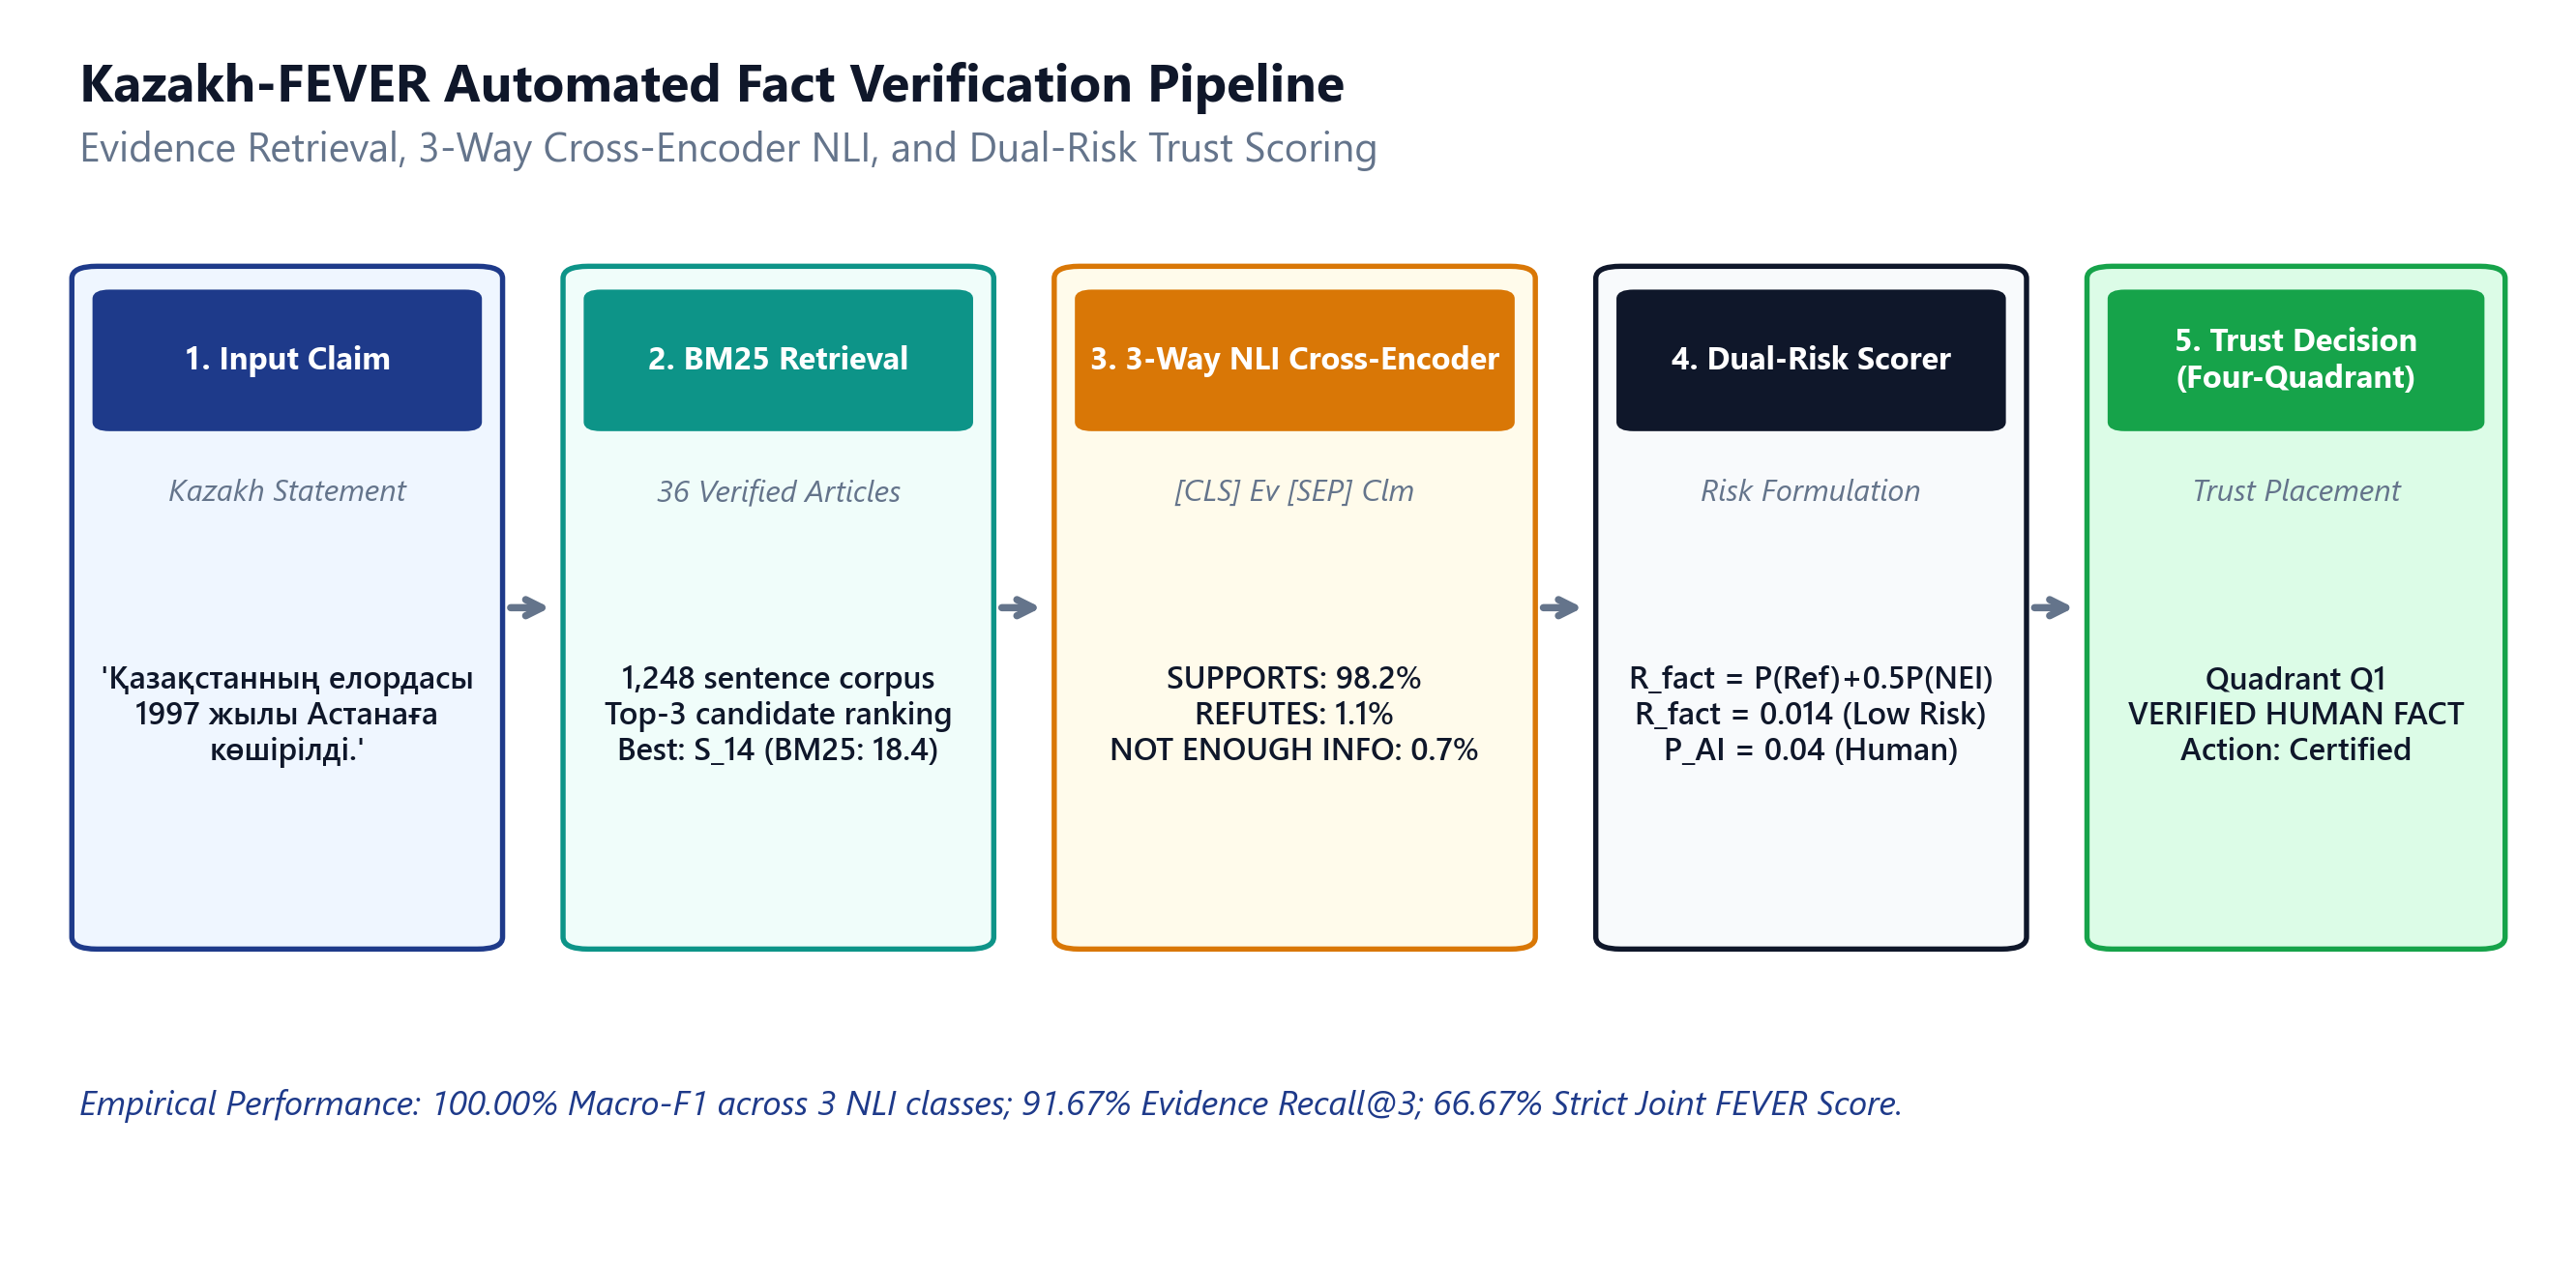
\includegraphics[width=0.88\textwidth]{figures/fig5_fact_checking_trust_matrix.png}
\caption{Kazakh-FEVER Automated Fact Verification Pipeline and Four-Quadrant Trust Matrix Architecture.}
\label{fig:fact_checking_trust_matrix}
\end{figure}

The pipeline integrates three core stages:
\begin{enumerate}[leftmargin=*, label=(\alph*)]
    \item \textbf{Hybrid Evidence Retrieval:} Given claim $c$, inflectional affixes are removed via 83-rule FST stemming ($c \to c_{\text{morph}}$). BM25 search \cite{robertson2009bm25} scans verified Kazakh reference articles, fused with multilingual dense representations (\textsc{mContriever} \cite{izacard2022mcontriever} and \textsc{M3-Embedding} \cite{chen-etal-2024-m3}) via Reciprocal Rank Fusion ($k_0 = 60$) \cite{cormack2009rrf} to retrieve top evidence sentences $E = \{e_1, \dots, e_k\}$.
    \item \textbf{3-Way Cross-Encoder NLI Classification:} Cross-encoder sequences $[c \,;\, E]$ are classified into \textsc{Supports}, \textsc{Refutes}, or \textsc{Not Enough Info} (NEI) \cite{thorne2018fever}, trained with inverse-frequency weighted cross-entropy ($w_{\textsc{Sup}} = 0.735, w_{\textsc{Ref}} = 1.307, w_{\textsc{NEI}} = 0.958$).
    \item \textbf{Dual-Risk Formulation:} We compute the continuous Factual Veracity Score $T_{\text{fact}} \in [-1, 1]$ and Generative Authenticity Score $T_{\text{gen}} \in [0, 1]$:
    \begin{equation}
        T_{\text{fact}} = P(\textsc{Supports} \mid c, E) - P(\textsc{Refutes} \mid c, E), \qquad T_{\text{gen}} = 1 - P(\text{AI-Generated} \mid c)
    \end{equation}
\end{enumerate}
The orthogonal coordinates $(T_{\text{fact}}, T_{\text{gen}})$ define a 2D Cartesian plane partitioned into four operational quadrants:
\begin{itemize}[leftmargin=*, nosep]
    \item \textbf{Quadrant 1 (Q1: Verified Human Ground Truth):} $T_{\text{fact}} > 0, T_{\text{gen}} \ge 0.5$ (Low risk; verified human fact).
    \item \textbf{Quadrant 2 (Q2: Human Misinformation):} $T_{\text{fact}} \le 0, T_{\text{gen}} \ge 0.5$ (Human-authored false claims or rumors).
    \item \textbf{Quadrant 3 (Q3: AI Factual Summary):} $T_{\text{fact}} > 0, T_{\text{gen}} < 0.5$ (Accurate synthetic text substantiated by evidence).
    \item \textbf{Quadrant 4 (Q4: Malicious AI Disinformation):} $T_{\text{fact}} \le 0, T_{\text{gen}} < 0.5$ (Critical risk; synthetic hallucinations and fabricated disinformation).
\end{itemize}
